\chapter[User-centric Payload Design for Sensor Placement]{User-centric Payload Design and Usability Testing for Agricultural Sensor Placement and Retrieval using Off-the-Shelf Micro Aerial Vehicles}
\label{ch:UR}

% Useful to reduce whitespace above/below figure, add in figure env., before/after \includegraphics
% \newcommand{\figurevspaceabove}{-0.6cm}
% \newcommand{\figurevspacebelow}{\vspace{-1.5em}}	
\newcommand{\figurevspacebelow}{\vspace{0em}}	

\author{Christian~Geckeler$^{1}$, Iris~Kong$^{1,2}$, and Stefano~Mintchev$^{1}$% <-this % stops a space
\thanks{This work was supported by the Swiss National Science Foundation through the Eccellenza Grant number 186865 (grant to S. Mintchev) and by Syngenta through the Plant Science Center-Syngenta Fellowship Program (grant to M. C. Schuman and S. Mintchev).}% <-this % stops a space
\thanks{$^{1}$The authors are with the Environmental Robotics Laboratory, Dep. of Environmental Systems Science, ETH Zurich, 8092 Zurich, Switzerland and with the Swiss Federal Institute for Forest, Snow and Landscape Research (WSL), 8903 Birmensdorf, Switzerland. {\tt\footnotesize \{cgeckeler, smintchev\}@ethz.ch}}
\thanks{$^{2}$ The author is also with the DTU Management Dep. of Technology, Management and Economics, Technical University of Denmark, Akademivej, Building 358, 2800 Kgs. Lyngby, Denmark. {\tt\footnotesize \{ickong\}@outlook.com} }%
}
% Alternate email: ickong@connect.ust.hk

% \thanks{$^{2}$Bernard D. Researcher is with the Department of Electrical Engineering, Wright State University,
%         Dayton, OH 45435, USA
%         {\tt\small b.d.researcher@ieee.org}}%

%% (RAL Final Version) Add more info lines in the \author command  (editor, accepted dates, etc)
%\author{Christian~Geckeler,
%	and Stefano~Mintchev%
%	\thanks{Manuscript received: July, 18, 2023; Revised October, 15, 2023; Accepted December, 12, 2023.}%Use only for final RAL version
%	\thanks{This paper was recommended for publication by Editor Hyungpil Moon upon evaluation of the Associate Editor and Reviewers' comments.
%		This work was supported by the Swiss National Science Foundation through the Eccellenza Grant number 186865.} %Use only for final RAL version
%	\thanks{The authors are with the Environmental Robotics Laboratory, Dept. of Environmental Systems Science, ETH Zurich, 8092 Zurich, Switzerland and with the Swiss Federal Institute for Forest, Snow and Landscape Research (WSL), 8903 Birmensdorf, Switzerland. {\tt\footnotesize \{cgeckeler, smintchev\}@ethz.ch}}%
%	\thanks{Digital Object Identifier (DOI): see top of this page.}
%}
%% Use only for final RAL version.

% \begin{document}
% \bstctlcite{BSTcontrol}


% \maketitle
% \thispagestyle{empty}	% Comment this line for final RAL version
% \pagestyle{empty}		% Comment this line for final RAL version

%% (Final RAL version) add Paper headers, fill in <name>
%\markboth{IEEE Robotics and Automation Letters. Preprint Version. <MONTH>, <YEAR>}
%{Geckeler \MakeLowercase{\textit{et al.}}: <TITLE>} 
%% Use only for final RAL version

%%%%%%%%%%%%%%%%%%%%%%%%%%%%%%%%%%%%%%%%%%%%%%%%%%%%%%%%%%%%%%%%%%%%%%%%%%%%%%%%
%%% Max 2250 characters
\begin{abstract}
Increased flight time and advanced sensors are making \glspl{MAV} easier to use, facilitating their widespread adoption in fields such as precision agriculture or environmental monitoring.
However, current applications are limited mainly to passive visual observation from far above; to enable the next generation of aerial robot applications, \glspl{MAV} must begin to directly physically interact with objects in the environment, such as placing and collecting sensors. Enabling these applications for a wide spectrum of end-users is only possible if the mechanism is safe and easy to use, without overburdening the user with complex integration, complicated control, or overwhelming and convoluted feedback.
To this end we propose a self-sufficient passive payload system to enable both the deployment and retrieval of sensors for agriculture. This mechanism can be simply mechanically attached to a commercial, off-the-shelf \gls{MAV}, without requiring further electrical or software integration. The user-centric design and mechanical intelligence of the system facilitates ease of use through simplified control with targeted perceptual feedback. 
%No separate controls for the payload are needed, through rigid attachment to the \gls{MAV}, already known \gls{MAV} control inputs position the mechanism for sensor deployment and collection. The integrated onboard \gls{MAV} camera, with added rearward facing camera, gives the user visual feedback on the state of collection or deployment.
The usability of the system is validated quantitatively and qualitatively in a user study demonstrating sensor deployment and collection. All participants were able to deploy and collect at least four sensors both within 10 minutes in visual line-of-sight and within 12 minutes in beyond visual line-of-sight, after only three minutes of practice. 
Enabling \glspl{MAV} to physically interact with their environment will usher in the next stage of \gls{MAV} utility and applications. Complex tasks, such as sensor deployment and retrieval, can be realized relatively simply, by relying on a mechanically passive system designed with the user in mind, these payloads can enable such applications to be more widely available and inclusive to end-users.
% utilizing already familiar control and visual feedback systems, these payloads can enable such applications to be more widely available and inclusive to end-users.
%By employing a user-centric and mechanically intelligent design, payloads can enable these applications to be more widely available and more inclusive to end-users.
\end{abstract}

% (RAL Final Version) only use keywords (max 5) then, check list: https://www.ieee-ras.org/publications/ra-l/keywords
% \begin{IEEEkeywords} %% only final version
% aerial sensor placement; environmental monitoring; forest canopies; micro-aerial vehicles;  Robotics and Automation in Agriculture and Forestry
% \end{IEEEkeywords}


%%%%%%%%%%%%%%%%%%%%%%%%%%%%%%%%%%%%%%%%%%%%%%%%%%%%%%%%%%%%%%%%%%%%%%%%%%%%%%%%
\section{Introduction}
% (RAL Final Version) Use only for final RAL version Formatting 
% Drop letter for first word of the Introduction
%\IEEEPARstart{F}{orests} 

Micro-aerial vehicles (\glspl{MAV}) are demonstrating increased utility in a widening array of applications, from standard remote sensing in agriculture \cite{Zhang2022}, to collecting and retrieving sensors \cite{Geckeler2022a, Geckeler2023a}. As a result, more and more \glspl{MAV} are piloted by end-users, who may not have a dedicated focus on piloting \glspl{MAV}. Advances in \gls{MAV} hardware and software, such as advanced attitude stabilization, omnidirectional obstacle avoidance, and low-latency, high resolution video feedback, have facilitated this transition; enhancing safety and reducing the complexity of piloting \glspl{MAV} so that more end-users can utilize this technology. Standard applications of \glspl{MAV} using visual sensors, such as mapping, photogrammetry, or detection of multispectral indices, are well established and straightforward for the end-user to conduct. Indeed, these tasks can already be partially or fully automated, requiring only the pilot's supervision during execution.

\begin{figure}[!t]
\centering
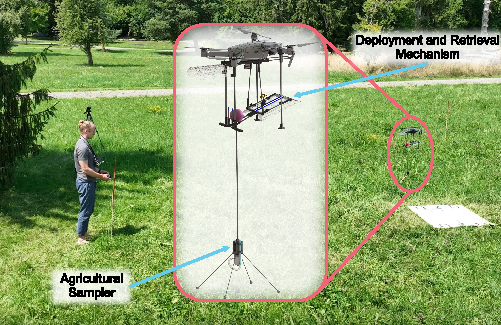
\includegraphics[width=1\columnwidth]{chapters/papers/UR/figures/fig-1-summary/fig-1-summary.pdf}
\caption{A user piloting the system to deploy a sensor on a target during the user study, detail shows the payload attached to the \gls{MAV} carrying a sensor.}
\label{fig:fig1-summary}
\figurevspacebelow
\end{figure}

The next stage for \gls{MAV} utility, however, will require \glspl{MAV} to move from visual sensing high above the region of interest, to direct, active physical interaction with the object of interest. \glspl{MAV} have begun to demonstrate utility in this direction for enhanced environmental monitoring, from physically collecting samples, be it environmental DNA by landing on branches \cite{Aucone2023a}, or cutting small twigs from the outer canopy\cite{Charron2020}, to placing and collecting sensors \cite{Geckeler2023a, Hamaza}. These more advanced applications of \glspl{MAV} are considerably more complex and carry greatly increased operational risk, requiring experienced pilots, oftentimes multiple pilots, one for the payload, and one for the MAV. While simple waypoint missions at high altitude with no risk of collision are easy to automate, introducing autonomy in these advanced tasks is more challenging, and a human pilot remains essential. The pilot brings cognitive flexibility to the task, from deciding where to place a specific sensor, to which sample needs to be collected, as well as invaluable accumulated experience. 
This includes an intuitive understanding of the scene, from detecting potential sources of collisions, to predicting the behavior of complex dynamic environments, such as elastic branches. 
%These are difficult to model and even more challenging to incorporate into a perception and control framework for a \gls{MAV}, but understandable for human pilot.

Therefore, we present a user-centric design for collecting and deploying ground-based sensors for crop monitoring in agricultural fields. The sensor deployment and collection mechanism is designed to be self-contained, so that it can be mounted on an off-the-shelf \gls{MAV} without requiring complicated mechanical, electrical, or software integration (Fig.~\ref{fig:fig1-summary}). Additionally, it is designed to be passive, so that no additional control burden falls on the pilot while also reducing the mechanical complexity of the design. The mechanism utilizes already known \gls{MAV} controls to collect and deploy sensors, and integrated cameras provide visual feedback. The main contributions of this work are as follows: a passive, user-friendly, payload design that can be mounted on an off-the-shelf \gls{MAV}, and a thorough user-study of six pilots on the usability of the mechanism, which demonstrates that this system can be reliably used by a single pilot to place and collect sensors for agriculture even after only three minutes of practice with the system. 

\section{Related Works}

\gls{MAV} use in precision agriculture for remote sensing is well established \cite{Zhang2022, Manfreda2018}, for instance to map plant stress using multispectral sensors. Recent work has begun to demonstrate \gls{MAV} use for tasks in agriculture and environmental monitoring which require closer proximity with the object of interest, including physical interaction. For instance, to attach sensors on tree branches \cite{Geckeler2022a, Geckeler2023BiodegradableBranches, Hamaza}, to place and collect samplers to detect plant stress from volatiles in agriculture \cite{Geckeler2023a}, or to collect physical samples. These physical samples include sampling environmental DNA by landing on branches\cite{Aucone2023a}, and physical samples by pruning leaves and twigs \cite{Kaslin2018, Charron2020, LaVigne2022, Krisanski2022}. These systems are either based on a custom \gls{MAV} platform which is not easily reproducible, or have a complex payload that is challenging to operate, requiring a dedicated pilot for the payload. While the authors in \cite{Krasylenko2023DruidManagement} present an array of attachments to small commercial, off-the-shelf \glspl{MAV} which enable the collection of physical samples, video recording, and spraying capabilities, a separate pilot is still necessary for operating the payload.

To deploy and retrieve sensors, a mechanism is needed to release and re-collect the sensor. In general existing approaches can be classified as active or passive, depending on whether an additional actuator is needed, or whether the mechanical design of the mechanism passively enables the collection and drop-off. Active systems have the benefit of usually being more controllable and precise, at the cost of the additional actuator, the power source, and increased control complexity. Active systems are also usually restricted to a singular object being grasped, limiting scalability. These systems include manipulators attached to \glspl{MAV}, performing dynamic or static grasping \cite{Ollero2022, Fishman2021, Kim2018c, Orsag2014, Suarez2017, Lee2021a, Roderick2021}, or enveloping the object to be grasped partially or fully with parts of the \gls{MAV} or with multiple \glspl{MAV} \cite{Hingston2020, Gabrich2018, Bamert, Zhao2017}.

Passive mechanisms benefit from reduced actuation complexity, which also usually brings with it weight savings and increased robustness, at the cost of limited controllability. A well-established method for aerial retrieval is using a hook which attaches to a suspended line or vice versa \cite{Leary, Geckeler2023a, Jiang2023}, as it is passive, robust, and does not require precise alignment. Other passive mechanisms include mechanically intelligent bistable grippers\cite{Firouzeh2023, Hsiao2022, Geckeler2022a}.

Despite the wealth of research on aerial grasping and manipulation using \glspl{MAV}, also for environmental monitoring and sample collection, the application in agriculture for sensor placement is limited. In our previous work \cite{Geckeler2023a}, we demonstrated a system to deploy and collect sampling pumps for volatile collection in agriculture. Plant volatiles are volatile compounds released by plants within seconds to hours after a stress event, enabling rapid detection of the type and severity plant stress, including insect herbivory. The system employed the hook and line method, which, while robust to misalignment, requires a complicated dynamic swooping manoeuvre. First, the \gls{MAV} must go forward while simultaneously remaining laterally aligned, then shortly afterwards also go upwards to engage the wire on the hook and prevent the sensor from tipping over or dragging on the ground. This proved quite challenging for the pilot, and the system needed a separate mechanism for the deployment and collection, while only being able to handle a single sampler at a time. Therefore, in this work we present a single passive mechanism, designed to be easy to use, which can attach to a small off-the-shelf \gls{MAV}, enabling collection and deployment of multiple sensors by a single pilot. 


\section{Methodology}

\begin{figure*}[!htp]
\centering
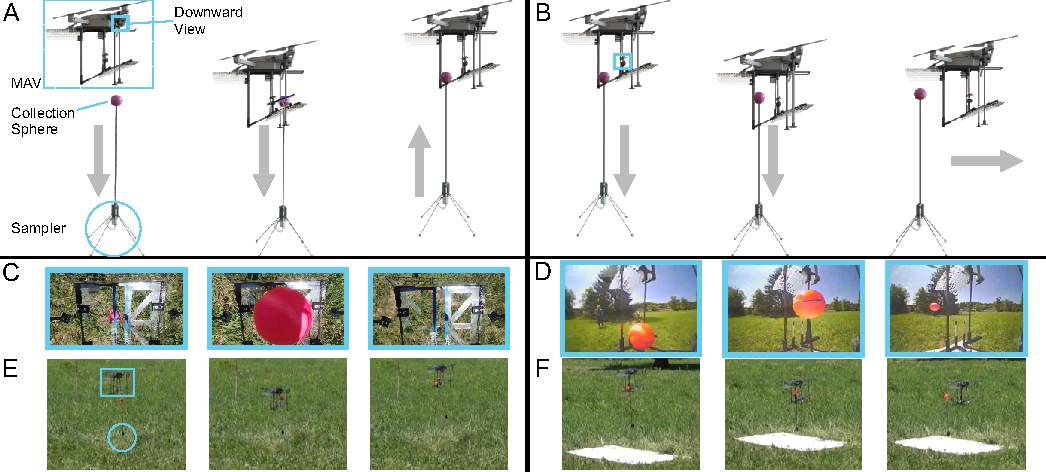
\includegraphics[width=\textwidth]{chapters/papers/UR/figures/fig-3a-working-principle/fig-3a-working-principle.pdf}
\caption{(A) Collection procedure: the \gls{MAV} centers on top of the sensor (A left), lowers until the sensor is collected by the trapdoor (A middle), then goes back up, which stores the sensor in the storage rack (A right). (B) Deployment procedure: the \gls{MAV} lowers (B left) until the sensor touches the ground and is above the drop-off pins (B middle), then the \gls{MAV} moves forward to clear the sensor (B right).  (C) Downward facing camera view from the main camera (blue box in (A)) during a user study. (D) Rearward facing camera view (blue box in (B)) during a user trial. (E) Sensor collection during user trials, (D) Sensor deployment on target during user trials. The grey arrows denote the \gls{MAV} commands required from the pilot during each phase.}
\label{fig:fig3a-working-principle}
\figurevspacebelow
\end{figure*}

The developed mechanism should attach to an off-the-shelf \gls{MAV} and enable a user to intuitively deploy and retrieve sensors for agriculture. This leads to the formulation of two types of requirements: human performance design considerations, and general requirements related to the hardware design and \gls{MAV} integration. The former should consider the strengths and limitations of the end-user, reducing control complexity while providing useful feedback.
General \gls{MAV} payload hardware design considerations include that the system should easily integrate into commercially available, off-the-shelf \glspl{MAV} using a simple mechanical coupling, without requiring further electrical or software integration. The system should be robust and incorporate safety mechanisms to reduce likelihood of compromising flight stability, and the design should be lightweight to maximize flight-time and allow deployment, retrieval, and transport of multiple sensors with the same mechanism.

From the perspective of the end-user, the task can be described as a teleoperated 3D positioning task, which ideally can also be completed \gls{BVLOS}, using only the onboard sensors and camera feeds.
%
This involves three main challenges, localization, alignment, and safe operation. 
Localization includes finding a suitable placement location for the sensor, using perhaps previously defined waypoints in addition to the onboard camera, as well as locating the sensor for recollection, for which it should be easily visible. 
The next challenge is alignment, both in terms of precision when deploying the sensor, ensuring that it is placed correctly and not on crops for instance, and in terms of fine control for pickup or deployment. The user must accurately control where the \gls{MAV} is in relation to the sensor to ensure proper deployment and collection, and must do so using only the limited perspectives provided by the onboard sensors. 
Lastly, to avoid a critical accident with the \gls{MAV}, the user should be supported for safe operations, e.g. to prevent the sensor from entering the propellers before collection or after deployment.
\newline
\indent We base our human performance design requirements on human performance principles from the field of Human Factors Engineering. Designing a \gls{MAV} payload attachment based on the capabilities, characteristics, and needs of people will improve human performance in terms of efficiency and safety \cite{Hobbs2016}. In general, the system should enable users to operate the system intuitively and effectively, even with only basic technical expertise or limited training. According to the human information processing model \cite{Wickens2021}, design changes can significantly affect human performance, and the human-robot (in this case MAV) interaction should optimize task speed, accuracy, and user attentional demands.
%
This necessitates that the required attentional demand and cognitive load of the user should be reduced as much as possible by offloading tasks through the incorporation of mechanically intelligent features and limiting the complexity of the system and its control. To reduce the difficulty of the task, we should improve teleoperator feedback \cite{Lathan2002} so that a greater sense of operator immersion can be achieved \cite{Burdea1996}. The real-time feedback system should provide the user only necessary information relevant to the task, enabling better situational awareness and decision making. Hardware limitations must also be considered, such as camera viewpoint and robot orientation, camera field of view, image resolution, depth perception, and latency for feedback and control \cite{Chen2007}. Since our system will integrate into a commercial \gls{MAV}, the feedback system will be highly reliant on the existing sensors and visual feedback from the camera system, which is also taken into consideration during the design process.

\subsection{Sensor Deployment and Retrieval Mechanism}

\subsubsection{Working Principle}

The basic working principle of the mechanism can be seen in Fig.~\ref{fig:fig3a-working-principle}, as well as the supplementary video.

The main components of the system (see Fig.~\ref{fig:fig2-hardware}) consist of an angled trapdoor mechanism to enable a passive one-way collection of the sensor, followed by parallel rails which constitute the storage rack, terminated by drop-off pins which also act as an end-stop for the stored sampler. Assuming a sensor is stored in the storage rack, a deployment procedure would proceed as follows (Fig.~\ref{fig:fig3a-working-principle}B): the user positions the \gls{MAV} above the target, slowly lowering the \gls{MAV} until the sensor touches the ground and the sphere attached to the sensor rises above the drop-off rods. Once the sphere has cleared the blue tips of the drop-off rods, as seen through the rearview camera, the \gls{MAV} moves forward and the sensor is deployed.

To retrieve the sensor after sampling, the user aligns the \gls{MAV} above the sensor sphere (Fig.~\ref{fig:fig3a-working-principle}A), lowering the \gls{MAV} while keeping the sphere centered in the camera view until the sphere has passed the trapdoor. The user then commands the \gls{MAV} to ascend vertically, where the sensor then slides back into the storage rack.

\subsubsection{Human Performance Design Considerations}

To address the first challenge of localization, the sensor sphere should be highly visible. By providing a large contrast against the background, a deployed sensor in the field can be identified faster and more robustly.
For trichromats (organisms with receptors in the eye for three colors, e.g. red, green, and blue) in a temperate forest environment, shades of red, magenta, and neon green are easiest to discern, whereas for dichromats, shades of blue, white, and yellow maximize visibility \cite{Fennell2019}. Since most humans are trichromats, a shade of fluorescent pink was chosen for the color of the sphere placed on top of the sensor. The fluorescence of the color has the added benefit of absorbing UV light beyond the visible spectrum and reflecting it at a lower, visible, wavelength. However, if the \gls{MAV} operator is dichromatic (color vision deficient), then a different color would provide greater visibility. 
% For a more inclusive system, future work should consider combining stripes of different colors to ensure enhanced visibility of the sphere for all users.

Alignment and positioning of the payload mechanism is made fast and intuitive by directly using the built-in \gls{MAV} control and perception system.
%By using the built in \gls{MAV} control and perception system to also directly position the payload mechanism, control is fast and intuitive for the pilot.
Since these controls and camera are already known by the pilot, it is easier to control the payload and judge the \gls{MAV} position and orientation relative to the sensor and environment. The lack of depth perception is compensated by providing alternate visual cues for the current state of deployment or retrieval, and reducing the needed precision. When the user deploys the sensor, the blue tips of the drop-off rods (Fig.~\ref{fig:fig2-hardware}) act as a vertical gauge of when the sphere has cleared them, and thus, when to begin moving forward (Fig.~\ref{fig:fig3a-working-principle}B, right)). This is easily judged through the added rear-facing \gls{FPV} camera (Fig.~\ref{fig:fig2-hardware}), which provides a clear view of the drop-off rods and sphere in the storage rack during deployment (captures of the viewpoint during a user-study can be seen in Fig.~\ref{fig:fig3a-working-principle}D).
During retrieval, the sphere must be centered in the camera frame, keeping it centered in the transparent trapdoor (Fig.~\ref{fig:fig3a-working-principle}C). The \gls{MAV} camera is positioned directly above the center of the trapdoor, facilitating intuitive alignment using the camera, since the user can simply follow the guidelines overlaid in the \gls{MAV} remote controller user interface (Fig.~\ref{fig:fig2-hardware}, Downward Main Camera view). The funnel around the trapdoor provides additional physical assistance in case of misalignment or drift. The cobalt blue edges of the trapdoor (Fig.~\ref{fig:fig2-hardware}) facilitate easy detection when the sphere is above the trapdoor, and when to stop lowering the MAV. To transfer the sensor in the storage rack, the user only has to move the \gls{MAV} up after collection. The angle of the trapdoor causes the sphere to automatically slide onto the storage rack and against the drop-off pins.

Lastly, to support the user in safe operations, propeller guards (Fig.~\ref{fig:fig2-hardware}) are added as an additional safety mechanism to reduce the likelihood of a \gls{MAV} crash as a result of user error. In the absence of propeller guards, if the \gls{MAV} is lowered further than necessary during deployment and moved forward, the sphere of the sensor may make contact with the rear propellers. Similarly during sensor collection, if the user continues to command the \gls{MAV} down after the sphere has entered the trapdoor, there is a possibility of the sphere entering the front propellers. To avoid these situations, an arched, single-sheet of fiberglass mesh is added in the rear and two parallel carbon rods in the front. Since the front propeller guard is under the camera, rods instead of a mesh are used to maintain downward visibility. To still provide the necessary safety, the rods are sized such that the sphere can neither pass through nor around them.

Reducing the complexity of the design to a passive system which is rigidly attached to the \gls{MAV} allows real-time, intuitive control, with no need for complicated control of a separate end-effector, nor the complex dynamics from a swinging attachment. Instead, both the control and visual feedback for positioning are identical with the \gls{MAV} controls, which the pilot is already familiar with. 

\subsubsection{Hardware Design}
\begin{figure}[!tp]
\centering
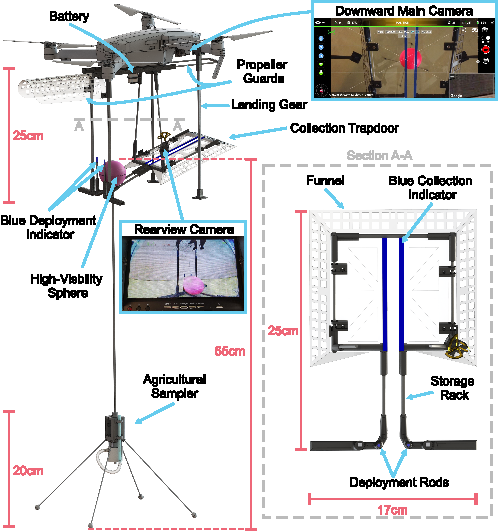
\includegraphics[width=0.9\columnwidth]{chapters/papers/UR/figures/fig-2-hardware/fig-2-hardware.pdf}
\caption{Components of the payload mechanism. The agricultural sampler is collected using the high-visibility sphere through the collection trapdoor, aided by the funnel. The blue lines on the collection trapdoor indicate when the sampler sphere has entered the trapdoor, as seen through the main, downward facing camera. During deployment, the blue tips of the deployment rods act as indicators when the \gls{MAV} is low enough to fly forwards, as seen through the rearview camera, powered through the onboard battery on the opposite side. Propeller guards in the front and rear provide additional protection during retrieval and collection. Note that the sampler sphere has been removed in the Section A-A view for enhanced clarity.}
\label{fig:fig2-hardware}
\figurevspacebelow
\end{figure}

The chosen \gls{MAV} was a DJI Mavic Pro, which, although not the newest \gls{MAV}, still has forward and downward obstacle detection, sensors for precise positioning and landing, as well as a gimbaled 4k main camera. To ascertain the maximum allowable weight of the mechanism, flight tests were performed with varying payload weights to measure the reduction in flight time as well as judge flight performance. With no additional payload, the battery reached 50\% after 11.35 minutes of continuous flight, with 400g of payload, this was reduced to 7.16 minutes. It should be noted that the manufacturer does not officially support additional payloads for this \gls{MAV}, which may result in reduced operational life, as evinced by the increased temperature of the motors after flight tests.

%114.25g = mechanism, 8.57g =battery, 4.5g = \gls{FPV} camera, rest is sampler?? 
%update: 139.38g (front landnig gear 16.56, battery 8.57, camera, trapdoor, storage rack, prop guards, etc 114.25, +sensor 72.16 => total 211.54 => flight itme
In total, the mechanism presented in Fig. \ref{fig:fig2-hardware} weighs 139.38g (front landing gear 16.56g, battery 8.57g, rest including trapdoor, camera, storage rack, and propeller guards 114.25), which, when combined with additional 72.16g for the sensor corresponds to 9 minutes of flight-time until the battery reaches 50\%. 
To keep the mechanism lightweight, main structural components are composed of carbon rods and beams, with joints and interfaces made from 3D printed ABS. Material for large areas, such as the rear propeller guard or trapdoor funnel is made from 0.3mm lasercut fiberglass. The trapdoor is laser-cut from 1mm clear poly methyl methacrylate (PMMA), to provide the necessary structural stability without reducing visibility. Additional material is removed from the trapdoor to reduce weight and air resistance. The five centimeter sensor sphere is made from 3D printed thermoplastic polyurethane, providing some damping and shock-absorption during collection. 
%% TODO weight breakdown
For the rear-view during deployment, a rear-facing \gls{FPV} camera is added, powered with a 1S 260mAh LiPo battery to remain self-sufficient mounted on the opposite side to balance the center of mass. An \gls{FPV} screen displaying the live feed from the camera (Fig.~\ref{fig:fig2-hardware}, rearview camera) was fitted with a lanyard so it could be suspended beside the regular \gls{MAV} remote control and display, providing the user with the rear-view beside the main gimbaled camera.
\\
\indent The storage rail in the center is designed to accommodate three of the sensor spheres, with the combined center of mass as close as possible to the \gls{MAV} center of mass. The sensor sphere acts as a ball joint for the sensor, which decouples oscillations of the sensor due to abrupt movements of the \gls{MAV} and improves overall stability when compared to rigidly attaching the sensor.  

% minimum sliding angle?
%20degree trapdoor angle

%prototype 5, 138.57g, 5cm TPU Sphere

\subsection{Experimental Setup}

To assess the usability of the system a user study was conducted. The study was designed to qualitatively assess the users' impressions of the system and quantitatively measure their performance. Both within visual line of sight (VLOS) and beyond visual line of sight (\gls{BVLOS}), the users were asked to collect and deploy as many sensors as possible, as accurately as possible, within a limited time period.


\begin{figure}[!t]
\centering
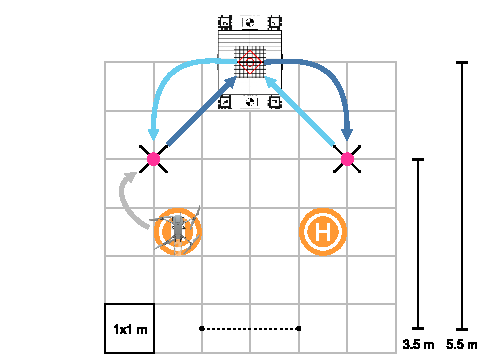
\includegraphics[width=0.8\columnwidth]{chapters/papers/UR/figures/fig-3-experimental-setup/fig-3-experimental-setup.pdf}
\caption{Experimental Setup: the user stands behind the dashed line, facing the target in VLOS tests and facing away during BVLOS tests. The \gls{MAV} starts on an orange landing pad, and the user can pick up one of the two sensors indicated by a pink sphere. After pickup, the user deploys the sensor on the target, after which the \gls{MAV} should ascend to four meters, wait until the sensor is cleared, and then continue with the next sensor. This repeats (dark blue and light blue arrows) until the time is up. Note that distances (gridlines) are to scale, but sizes (target, \gls{MAV}, samplers) are not.}
\label{fig:fig3-experimental-setup}
\figurevspacebelow
% \vspace{-2em}
\end{figure}

The experimental setup is shown in Fig. \ref{fig:fig3-experimental-setup}. Experiments were conducted outside in an open field; two sensors were placed four meters apart, 3.5m from the pilot and 2.5m from the target. Shorter distances were chosen since the main difficulty lies in the actual collection and deployment procedure, but also to facilitate the number of pick-ups and drop-offs within the limited time. The \gls{MAV} starts on one of the take-off spots, then the user collects a sensor, goes to the target, and deploys it. After deployment, the user flies up to four meters, the position of the sensor is marked, the sensor is reset, and then the pilot can continue with the second sensor. 

Each participant conducted the study individually with the following procedure: a 15 minute introduction gave an overview of the system, the aims of the project, safety features, and the experimental tasks. This includes a video demonstration of the pickup and drop-off procedure. 
The participant starts with a three minute practice round to get familiar with the \gls{MAV} controls and to practice a pickup and drop-off. Then there are two \gls{VLOS} flight tests of five minutes, with a three minute break in between. Next, the participant conducts the \gls{BVLOS} tests, with two flights of six minutes and a three minute break in between. The questionnaire is filled out after the introduction, and after both the \gls{VLOS} and \gls{BVLOS} flight tests.

% essentially two 5 min \gls{VLOS}, 2 6 min \gls{BVLOS}, and a 3 min practice and the start.

In the \gls{VLOS} tests, the pilot can directly visually observe the \gls{MAV} and sensor, thus perceiving a third-person view of the environment, with increased situational awareness. During \gls{BVLOS} tests, the pilot relies purely on the onboard sensors, the first-person view provided by the main \gls{MAV} camera, and the additional rear-view camera for deploying the sensors. By assessing the time taken to place and collect the sensors, the accuracy of placement, and the difference between the \gls{VLOS} and \gls{BVLOS} experiments  the performance of the system can be measured. After each experiment, users were asked to complete a questionnaire to understand their opinion of the system and its performance. The first ten questions in the questionnaire follow the System Usability Scale (SUS) \cite{Brooke1996}, and the rest verified design assumptions. The final part of the questionnaire contained open-ended questions to provide additional insights on the users' opinion of the system.


% pickup metricrs:
% - time required for sensor pickup
% - number of successful collection attempts vs misses (required reset of drone), also knocking over
% dropoff metrics:
% -time required to deploy sensor
% -accuracy on target  (+ # fall over)



\section{Experimental Results}

% weather correlation analysis (which metric??)

Six study participants were recruited, and to ensure safe operation of the \gls{MAV} and comply with regulations, each participant was required to possess a valid UAV license according to the European Union Aviation Safety Agency (EASA). Future end-users must also have such a license to fly the \gls{MAV} to comply with legal regulations. All participants are male, between the ages of 23 and 37, and when asked about \gls{MAV} flying experience on a scale of 1 to 10 (ten highest), the responses ranged from 6 to 8. 

\subsubsection{Retrieval}

\begin{figure}[!t]
\centering
% \begin{tikzpicture}  [align=center]
%   \begin{axis}
%     [boxplot/draw direction = x,
%     xmajorgrids,
%     minor x tick num=1,
%     xminorgrids,
%     y dir=reverse, %to have round1 at the top
%     % ymajorgrids,
%     boxplot/box extend=0.4, %control width of boxplot box
%     height=0.5\columnwidth,
%     width= \columnwidth,
%     ytick={1,2,3,4},
%     yticklabels={Round 1, Round 2, Round 3, Round 4},
%     xlabel={Time per Collection Attempt (s)},
%     % nodes near coords,
%     cycle list ={m-blue, m-green, m-red, m-cyan, m-yellow},
%     every axis plot/.append style={thick, fill, fill opacity =0.5}
%     ]
%   \foreach \n in {0,...,3} {
% 			\addplot+[boxplot, mark=*, fill, draw=black] table[y index=\n, col sep=comma] {figures/fig-4-retrieval/retrieval-time.csv};
% 		};
%   \end{axis}
% \end{tikzpicture}

\begin{tikzpicture}  [align=center]
  \begin{axis}
    [customboxplotstyle, xlabel={Time per Collection Attempt (s)},]
  \foreach \n in {0,...,3} {
			\addplot+[customaddplotstyle] table[y index=\n, col sep=comma] {chapters/papers/UR/figures/fig-4-retrieval/retrieval-time.csv};
		};
  \end{axis}
\end{tikzpicture}
\vspace{-0.6em}
\caption{Average time taken taken for all participants per collection attempt, per round.}
\label{fig:fig4-retrieval-time-boxplot}
\end{figure}

\begin{figure}[!t]
\centering
\begin{tikzpicture}  [align=center]
  \begin{axis}
    [customboxplotstyle, xlabel={Number of Collections},]
  \foreach \n in {0,...,3} {
			\addplot+[customaddplotstyle] table[y index=\n, col sep=comma] {figures/fig-4-retrieval/retrieval-number.csv};
		};
  \end{axis}
\end{tikzpicture}
\vspace{-0.6em}
\caption{Number of pick-ups per round.}
\label{fig:fig4-retrieval-number-boxplot}
\end{figure}

%% maybe figure with pointcloud of average deployment locations

In total, there were four flight experiments for each participant, two in \gls{VLOS}, and two \gls{BVLOS}. Fig. \ref{fig:fig4-retrieval-time-boxplot} shows the average time taken per collection attempt per round, and Fig. \ref{fig:fig4-retrieval-number-boxplot} shows the average number of  collection attempts per round, per person. Fig.~\ref{fig:fig4-retrieval-time-boxplot} shows that in Round 3, the first \gls{BVLOS} round, there was a significant increase in the average time needed to collect a sensor, indicating that despite two rounds in \gls{VLOS}, the \gls{BVLOS} is still more challenging. In round 4, the final \gls{BVLOS} round, the collection times stabilize again, indicating that with practice \gls{BVLOS} performance can become comparable to \gls{VLOS}.
The average time for each of the four rounds was 25.04s, 25.76s, 50.00s, and 31.41s, respectively. 

%%timing with misses + computation

\subsubsection{Deployment}

\begin{figure}[!t]
\centering
% \definecolor{m-blue}    {HTML}{4477AA}
% \definecolor{m-cyan}    {HTML}{66CCEE}
% \definecolor{m-green}   {HTML}{228833}
% \definecolor{m-yellow}  {HTML}{CCBB44}
% \definecolor{m-red}     {HTML}{EE6677}
% \definecolor{m-purple}  {HTML}{AA3377}
% \definecolor{m-grey}    {HTML}{BBBBBB}
 
% % \begin{tikzpicture}  [align=center]
% %   \begin{axis}
% %     [boxplot/draw direction = y,
% %     xtick={1,2,3, 4},
% %     xticklabels={Round 1, Round 2, Round 3, Round 4},
% %     cycle list ={m-blue, m-green, m-red, m-cyan, m-yellow},
% %     every axis plot/.append style={thick, fill, fill opacity =0.5,  boxplot/outlier={mark=*}}
% %     ]
% %     \addplot+[
% %     boxplot prepared={
% %       median=26,
% %       upper quartile=32,
% %       lower quartile=14.5,
% %       upper whisker=56,
% %       lower whisker=6
% %     },
% %     ] coordinates {};
% %     \addplot+[
% %     boxplot prepared={
% %       median=20,
% %       upper quartile=34.5,
% %       lower quartile=11.5,
% %       upper whisker=80,
% %       lower whisker=8
% %     },
% %     ] coordinates {};
% %     \addplot+[
% %     boxplot prepared={
% %       median=43.5,
% %       upper quartile=60.25,
% %       lower quartile=37.5,
% %       upper whisker=85,
% %       lower whisker=33
% %     },
% %     ] coordinates {};
% %     \addplot+[
% %     boxplot prepared={
% %       median=24.75,
% %       upper quartile=43,
% %       lower quartile=15,
% %       upper whisker=75,
% %       lower whisker=9
% %     },
% %     ] coordinates {};
% %   \end{axis}
% % \end{tikzpicture}

% % \begin{filecontents*}{data.csv}
% % 23	36	53	18
% % 46	8	47	44
% % 9	19	44	19
% % 34	34	35	43
% % 17	11	27	39
% % 14	33	34	23
% % 24	20	13	19
% % 24	22	32	19
% % 13	13	20	12
% % 34	13	33	17
% % 14	16	33	33
% % 24	16	58	21
% % 15	17	50	26
% % 16	18		18
% % 16	16		19.5
% % 15	19		29.5
% % 17	14		30
% % 19	56		22
% % 20	41		
% % 42	14		
% % 13	19		
% % \end{filecontents*}


% % \begin{tikzpicture} [align=center]
% \begin{tikzpicture} [align=center]
% 	% \pgfplotstableread[col sep=comma]{data.csv}\csvdata
%  	% \pgfplotstabletranspose\datatransposed{\csvdata} 
%   \begin{axis}
%     [boxplot/draw direction = y,
%     ymajorgrids,
%     minor y tick num=1,
%     yminorgrids,
%     % xmajorgrids,
%     xtick={1,2,3,4},
%     xticklabels={Round 1, Round 2, Round 3, Round 4},
%     ylabel={Time per Collection Attempt (s)},
%     % nodes near coords,
%     cycle list ={m-blue, m-green, m-red, m-cyan, m-yellow},
%     every axis plot/.append style={thick, fill, fill opacity =0.5}
%     ]
% 		\foreach \n in {0,...,3} {
% 			\addplot+[boxplot, mark=*, fill, draw=black] table[y index=\n, col sep=comma] {figures/fig-5-deployment/deployment-time.csv};
% 		};
%   \end{axis}
% \end{tikzpicture}


% % \begin{tikzpicture}  [align=center]
% % 	\pgfplotstableread[col sep=comma]{figures/fig-5-deployment/deployment_time.csv}\csvdata
% %  	\pgfplotstabletranspose\datatransposed{\csvdata} 
% %   \begin{axis}
% %     [boxplot/draw direction = y,
% %     xtick={1,2,3,4},
% %     xticklabels={Round 1, Round 2, Round 3, Round 4},
% %     cycle list ={m-blue, m-green, m-red, m-cyan, m-yellow},
% %     every axis plot/.append style={thick, fill, fill opacity =0.5}
% %     ]
% % 	\foreach \n in {1,...,4} {
% % 	   \addplot+[boxplot, mark=*, fill, draw=black] table[y index=\n, col sep=comma] {figures/fig-5-deployment/deployment_time.csv};
% %     };
% %  	% \foreach \n in {1,...,4} {
% % 	 %   \addplot+[boxplot, mark=*, fill, draw=black] table[y index=\n, col sep=comma] {datatransposed};
% %   %   };
% %   \end{axis}
% % \end{tikzpicture}


\begin{tikzpicture} [align=center]
  \begin{axis}
    [customboxplotstyle, xlabel={Time per Deployment Attempt (s)},]
  \foreach \n in {0,...,3} {
			\addplot+[customaddplotstyle] table[y index=\n, col sep=comma] 
   {figures/fig-5-deployment/deployment-time.csv};
		};
  \end{axis}
\end{tikzpicture}
\vspace{-0.6em}
\caption{Average time taken for all participants per deployment attempt, per round.}
\label{fig:fig5-deployment-time-boxplot}
\end{figure}

\begin{figure}[!t]
\centering
% \definecolor{m-blue}    {HTML}{4477AA}
% \definecolor{m-cyan}    {HTML}{66CCEE}
% \definecolor{m-green}   {HTML}{228833}
% \definecolor{m-yellow}  {HTML}{CCBB44}
% \definecolor{m-red}     {HTML}{EE6677}
% \definecolor{m-purple}  {HTML}{AA3377}
% \definecolor{m-grey}    {HTML}{BBBBBB}

% \begin{tikzpicture}  [align=center]
% 	% \pgfplotstableread[col sep=comma]{data.csv}\csvdata
%  	% \pgfplotstabletranspose\datatransposed{\csvdata} 
%   \begin{axis}
%     [boxplot/draw direction = y,
%     ymajorgrids,
%     minor y tick num=1,
%     yminorgrids,
%     % xmajorgrids,
%     xtick={1,2,3,4},
%     xticklabels={Round 1, Round 2, Round 3, Round 4},
%     ylabel={Time per Collection Attempt (s)},
%     % nodes near coords,
%     cycle list ={m-blue, m-green, m-red, m-cyan, m-yellow},
%     every axis plot/.append style={thick, fill, fill opacity =0.5}
%     ]
% 		\foreach \n in {0,...,3} {
% 			\addplot+[boxplot, mark=*, fill, draw=black] table[y index=\n, col sep=comma] {figures/fig-5-deployment/deployment-number.csv};
% 		};
%   \end{axis}
% \end{tikzpicture}

\begin{tikzpicture} [align=center]
  \begin{axis}
    [customboxplotstyle, xlabel={Number of Deployments},]
  \foreach \n in {0,...,3} {
			\addplot+[customaddplotstyle] table[y index=\n, col sep=comma] 
   {chapters/papers/UR/figures/fig-5-deployment/deployment-number.csv};
		};
  \end{axis}
\end{tikzpicture}
\vspace{-0.6em}
\caption{ Number of drop-offs per round.}
\label{fig:fig5-deployment-number-boxplot}
\end{figure}

\begin{figure}[!t]
\centering
% \definecolor{m-blue}    {HTML}{4477AA}
% \definecolor{m-cyan}    {HTML}{66CCEE}
% \definecolor{m-green}   {HTML}{228833}
% \definecolor{m-yellow}  {HTML}{CCBB44}
% \definecolor{m-red}     {HTML}{EE6677}
% \definecolor{m-purple}  {HTML}{AA3377}
% \definecolor{m-grey}    {HTML}{BBBBBB}

% \begin{tikzpicture}  [align=center]
% 	% \pgfplotstableread[col sep=comma]{data.csv}\csvdata
%  	% \pgfplotstabletranspose\datatransposed{\csvdata} 
%   \begin{axis}
%     [boxplot/draw direction = y,
%     ymajorgrids,
%     minor y tick num=1,
%     yminorgrids,
%     % xmajorgrids,
%     xtick={1,2,3,4},
%     xticklabels={Round 1, Round 2, Round 3, Round 4},
%     ylabel={Time per Collection Attempt (s)},
%     % nodes near coords,
%     cycle list ={m-blue, m-green, m-red, m-cyan, m-yellow},
%     every axis plot/.append style={thick, fill, fill opacity =0.5}
%     ]
% 		\foreach \n in {0,...,3} {
% 			\addplot+[boxplot, mark=*, fill, draw=black] table[y index=\n, col sep=comma] {figures/fig-5-deployment/deployment-accuracy.csv};
% 		};
%   \end{axis}
% \end{tikzpicture}

\begin{tikzpicture} [align=center]
  \begin{axis}
    [customboxplotstyle, xlabel={Deployment Accuracy (cm)},]
  \foreach \n in {0,...,3} {
			\addplot+[customaddplotstyle] table[y index=\n, col sep=comma] 
   {figures/fig-5-deployment/deployment-accuracy.csv};
		};
  \end{axis}
\end{tikzpicture}
\vspace{-0.6em}
\caption{The accuracy, distance to target center, per round.}
\label{fig:fig5-deployment-accuracy-boxplot}
\end{figure}

Fig. \ref{fig:fig5-deployment-time-boxplot} shows the time taken per deployment, Fig. \ref{fig:fig5-deployment-number-boxplot} the number of attempts, and Fig. \ref{fig:fig5-deployment-accuracy-boxplot} the average distance of the deployed sampler to the center of the target. The time taken per deployment follows a similar trend as for collection, with an increase in the time taken for round 3, and then again an improvement down to previous levels in round 4. For all deployment attempts, the sensor always landed within 56cm of the target, with the average for each of the four rounds being: 17.4cm, 20.2cm, 16.9cm, and 15.7cm respectively.
The accuracy of sensor deployment does not vary significantly between the rounds, indicating that the \gls{BVLOS} feedback system provided a similar level of information to the user as when flying \gls{VLOS}. The average error for all rounds was 17.56cm. The closest deployments per round were 2.3cm, 1.8cm, 1.8cm, and 2.6cm, respectively, indicating that the system also allows for very accurate placement under favourable conditions.

\subsubsection{Questionnaire Results}
For the full questions and Likert Scale of the responses for the VLOS and BVLOS questionnaires, see the supplementary materials \cite{Geckeler}.
Some opinions were clearly shared between all participants for all flights; for instance, the high visibility of the pink sphere within the camera view, being able to identify when the sensor has touched the ground, and remembering to fly up after the sphere has passed the trapdoor. 

All participants found \gls{MAV} stability inconsistent, with lateral drifting, especially with wind. This made positioning and aligning with the sensor more challenging and time-consuming. Many participants lost visibility of the \gls{FPV} monitor due to poor connection, and some participants relied on other visual cues within the main camera view, such as the shadow of the sensor for deployment.


\begin{figure}[!t]
\centering
% \begin{tikzpicture} [align=center]
%   \begin{axis}
%     [customboxplotstyle, xlabel={Time per Deployment Attempt (s)},]
%   \foreach \n in {0,...,3} {
% 			\addplot+[customaddplotstyle] table[y index=\n, col sep=comma] 
%    {figures/fig-6-bvlos-vlos/sus-bvlos-vlos.csv};
% 		};
%   \end{axis}
% \end{tikzpicture}

% \begin{tikzpicture}  [align=center]
%   \begin{axis}
%     [boxplot/draw direction = x,
%     xmajorgrids,
%     minor x tick num=1,
%     xminorgrids,
%     y dir=reverse, %to have round1 at the top
%     % ymajorgrids,
%     boxplot/box extend=0.1, %control width of boxplot box
%     height=0.25\columnwidth,
%     width= \columnwidth,
%     % ytick={1},
%     % yticklabels={Round 1, Round 2, Round 3, Round 4},
%     yticklabel=\empty,
%     xlabel={Percent Difference in SUS Score BVLOS to VLOS},
%     % nodes near coords,
%     cycle list ={m-blue, m-green, m-red, m-cyan, m-yellow},
%     every axis plot/.append style={thick, fill, fill opacity =0.5}
%     ]
%   \addplot+[boxplot, mark=*, fill, draw=black] table[y index=0, col sep=comma] {figures/fig-6-bvlos-vlos/sus-bvlos-vlos.csv};
%   \end{axis}
% \end{tikzpicture}

\begin{tikzpicture}  [align=center]
  \begin{axis}
    [customboxplotstyle,
    height=0.25\columnwidth,
    xlabel={Percent Difference in SUS Score BVLOS to VLOS},
    xmin=-0.3,
    xmax=0.3,
    yticklabels={},
    ]
  \addplot+[boxplot, mark=*, fill, draw=black] table[y index=0, col sep=comma] {chapters/papers/UR/figures/fig-6-bvlos-vlos/sus-bvlos-vlos.csv};
  \end{axis}
\end{tikzpicture}
\caption{Difference in percent of the SUS score of all users between the \gls{BVLOS} and \gls{VLOS} rounds.}
\label{fig:fig6-bvlos-vlos}
% \figurevspacebelow
\end{figure}

In the \gls{BVLOS} setting, users found it easy to locate and navigate to the sensor and the target. A surprising result when comparing the \gls{VLOS} and \gls{BVLOS} tests was that not all participants found the \gls{VLOS} easier than the \gls{BVLOS}. Instead, two out of six found the \gls{BVLOS} easier and one found it equally challenging. This was not reflected in the number of retrieval and deployment sequences per minute between \gls{VLOS} and \gls{BVLOS}, where all participants took longer in \gls{BVLOS} compared to \gls{VLOS}. The first ten questionnaire questions are weighted to compute the SUS score, which is compared \gls{BVLOS} and \gls{VLOS} (Fig.~\ref{fig:fig6-bvlos-vlos}, average for all users), the system was more usable in \gls{VLOS} than \gls{BVLOS}, although there is a large deviation between users. For some participants with a significantly lowers SUS score for \gls{BVLOS} than \gls{VLOS} there was also a more significant difference between the number of sequences per minute.

Due to \gls{MAV} stability, all participants found it difficult to position the trapdoor above the sensor, however, once aligned, all found it reliable. In the \gls{VLOS} case, a third of the participants found the blue lines on the trapdoor helpful, a third found it unhelpful, and a third were indifferent, possibly since the participants relied less on the camera view during the \gls{VLOS} case. In the \gls{BVLOS} case, the majority found it helpful. All found that the blue lines on the trapdoor did not obstruct the view below.
More than half found it difficult to position the sphere vertically for deployment before flying forward in \gls{VLOS}, but found it easier in \gls{BVLOS}. This could be due to increased practice with the system, or increased reliance on the rear-facing \gls{FPV} monitor.
The blue tips for deployment were helpful to some in \gls{VLOS}, but moreso in \gls{BVLOS}, especially if used with the \gls{FPV} monitor.
Most people found manual take-off and landing with the \gls{MAV} and payload easy in \gls{VLOS}. In \gls{BVLOS}, most found landing easy, and half found the take-off easy, whereas the rest found it moderately easy or slightly difficult.

% for full questionnaire and results, see supplementary materials



\section{Discussion}

The user study demonstrated that all participants could deploy and collect at least four sensors with the mechanism, after only a few minutes of practice. However, for more robust conclusions, the user study could be improved.

First, the demographic of the participants is highly skewed, all work in some capacity with \glspl{MAV}, thereby having more experience than the average casual hobbyist pilot; also, all are male which introduces additional biases. A larger, more diverse, and more representative user-study should be conducted to provide more conclusive data that the mechanism is indeed usable by a wider audience. The color of the sensor sphere was chosen to be highly visible for trichromats; for a more inclusive system, future work should consider combining stripes of different colors to ensure enhanced visibility for all users, including for people with color vision deficiencies. Since the user-study took place over several days, environmental conditions, especially wind speed and gusts, changed. While no correlation between performance and weather was found, controlling for this variable would yield more conclusive data. All users easily located the sensor, which was in part due to the small test setup, since the \gls{MAV} was never more than six meters from a sensor. However, in a larger field, waypoint navigation could be used to bring the \gls{MAV} to the approximate location of sensor deployment, which would again create similar conditions.  
Lastly, participants were already more familiar with the system when starting the \gls{BVLOS} trials, since the \gls{BVLOS} trials were conducted after two rounds of \gls{VLOS} trials; future user-studies should randomize the order to correct this.

The largest complaint when flying the \gls{MAV} was stability, since the \gls{MAV} was prone to drift and difficult to keep steady with the added payload. This can easily be rectified by using a newer or larger \gls{MAV} with a greater carrying capacity, such as the Mavic 3.
The sensor, especially with the weight of the added sphere on top is quite top heavy, which can cause it to tip over during collection. This should be optimized to shift the center of mass down and reduce the likelihood of it falling over, while balancing the need to keep the center of mass close to the MAV.

User opinion on the additional rear-facing \gls{FPV} monitor was divided, with two-thirds being indifferent or finding it unhelpful in the \gls{VLOS} tests, but the majority found it helpful in the \gls{BVLOS} tests. Since this camera needs an additional power source (combined adding 13.1g), as well as an additional screen for viewing, it would be better to remove these components and integrate this view directly into the main \gls{MAV} perception system. This can be accomplished either by using a different \gls{MAV} where the camera can look further back (e.g. Parrot Anafi Ai \cite{ParrotWhitepaper}, whose main camera can pitch -116 to 176 degrees) or by adding a small mirror which provides this perspective in the main camera.

Autonomous take-off and landing with the attached payload has been successfully tested. In combination with waypoint navigation, this only requires the human pilot to perform the deployment and retrieval of the sensors. In the future, this can also be automated, simplifying the pilot's task to that of supervision, similar to current autonomous mapping flights. Interestingly, the considerations and design choices made to allow for easy human usability of the system also facilitates easier automation. Successful \gls{BVLOS} operations using only onboard sensors were demonstrated, showcasing that all necessary feedback is already available. Cameras for visual servoing have the right field of view, the sphere is highly visible for computer vision algorithms, and there are clearly defined control transitions for the different phases of the deployment and retrieval. The transitions are identical to the cues followed by the pilots, for the collection, the \gls{MAV} should keep the sphere centered within the trapdoor until the it has passed the blue lines, at which point the \gls{MAV} should go up; for the deployment the \gls{MAV} should descend until the sphere is above the blue tips of the deployment rods, then go forward. 

\section{Conclusion}

This work has demonstrated a self-sufficient, mechanically intelligent mechanism which can be attached to an off-the-shelf commercially available \gls{MAV} to enable collection and deployment of sensors for agricultural monitoring. The mechanism can be easily mechanically attached to the \gls{MAV}, requiring no further integration. Through user-centric design, the mechanism is easy and intuitive to use, as validated through a user study. In the user study, participants performed as many consecutive collections and deployments as possible, as accurately as possible, both within \gls{VLOS} and \gls{BVLOS}. All participants could execute at least four sensor collections and deployments both within 10 min \gls{VLOS}, and  also within 12min \gls{BVLOS}, after only three minutes of practice. The sensors were also deployed accurately, with the average distance from the center of the target being 17.56cm. The qualitative assessment through the questionnaire confirmed the usability of the system,  indicating that it was intuitive to use and that the visual cues chosen for the different deployment and retrieval states were helpful for the task.

For the next stage of \gls{MAV} utility, they will need to interact with objects in their environment, such as placing and collecting sensors. To ensure adoption into the field by end-users, such as for environmental or agricultural monitoring, these systems should be intuitive and easy to use. Through a user-centric design approach, the mechanism can be made both user-friendly and easily automatable for the future.

%Needed? or \vfill?
% \addtolength{\textheight}{-12cm}   % This command serves to balance the column lengths
                                  % on the last page of the document manually. It shortens
                                  % the textheight of the last page by a suitable amount.
                                  % This command does not take effect until the next page
                                  % so it should come on the page before the last. Make
                                  % sure that you do not shorten the textheight too much.

%%%%%%%%%%%%%%%%%%%%%%%%%%%%%%%%%%%%%%%%%%%%%%%%%%%%%%%%%%%%%%%%%%%%%%%%%%%%%%%%


%%%%%%%%%%%%%%%%%%%%%%%%%%%%%%%%%%%%%%%%%%%%%%%%%%%%%%%%%%%%%%%%%%%%%%%%%%%%%%%%


%%%%%%%%%%%%%%%%%%%%%%%%%%%%%%%%%%%%%%%%%%%%%%%%%%%%%%%%%%%%%%%%%%%%%%%%%%%%%%%%
%\section*{APPENDIX}
%Appendixes should appear before the acknowledgment.

\section*{Acknowledgment}

The authors would like to thank all study participants and to also extend their thanks to Ole Ravn for assisting with supervision during the thesis work.

%%%%%%%%%%%%%%%%%%%%%%%%%%%%%%%%%%%%%%%%%%%%%%%%%%%%%%%%%%%%%%%%%%%%%%%%%%%%%%%%

% \bibliographystyle{bibtex/IEEEtran}
% \bibliography{bibtex/references.bib,bibtex/control}

% \end{document}
